\chapter{Mediciones y resultados}
En este capítulo se presentan los resultados obtenidos del diseño del protocolo SPI, utilizado para controlar los convertidores D/A y A/D, así como la caracterización de las fotorresistencias. Además, se incluyen las imágenes obtenidas por medio de la matriz de fototransistores.


\section{Resultados de protocolo SPI}

\subsection{ADC}

            \begin{figure}[hbtp]
                \centering
                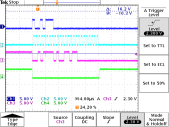
\includegraphics[width=0.6\textwidth]{ss_osc_adc_2v}
                \caption{Captura de osciloscopio de lectura y escritura de ADC.}
                \label{fig:ss_osc_adc_2v}
            \end{figure} 

            \begin{figure}[hbtp]
                \centering
                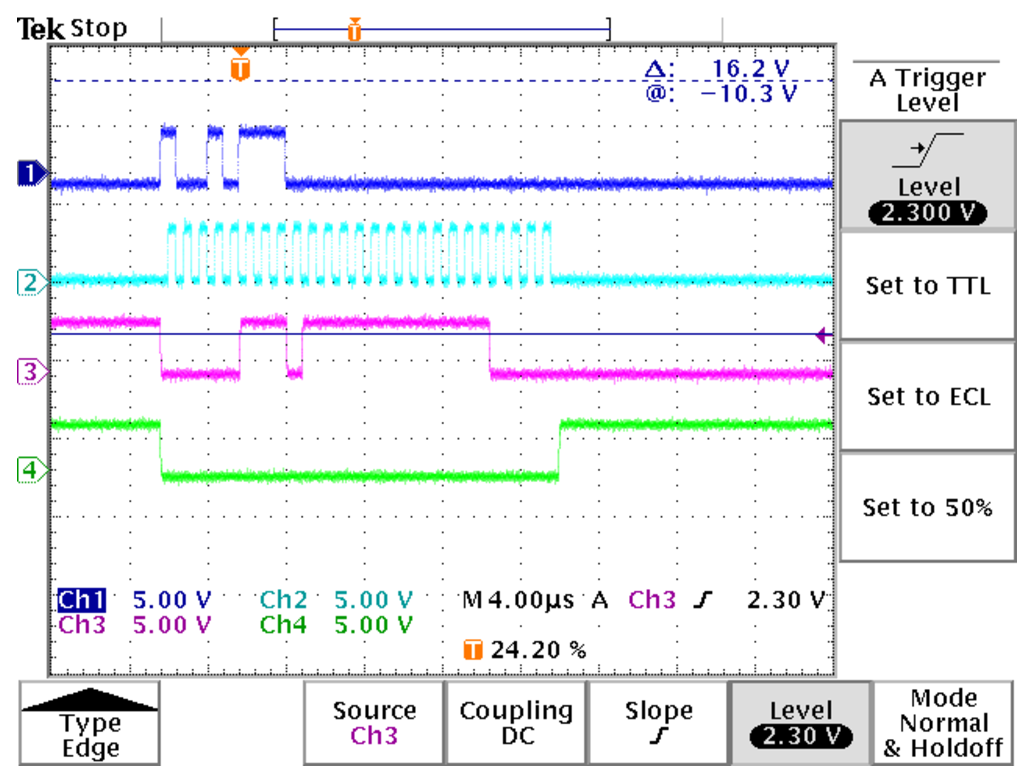
\includegraphics[width=0.6\textwidth]{ss_osc_adc_3v}
                \caption{Captura de osciloscopio de lectura y escritura de ADC.}
                \label{fig:ss_osc_adc_3v}
            \end{figure} 

\newpage     
\subsection{DAC}

            \begin{figure}[hbtp]
                \centering
                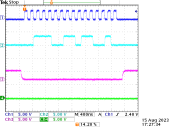
\includegraphics[width=0.6\textwidth]{ss_osc_dac_2v}
                \caption{Captura de osciloscopio de lectura y escritura de DAC.}
                \label{fig:ss_osc_dac_2v}
            \end{figure}
            
            \begin{figure}[hbtp]
                \centering
                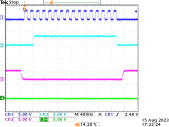
\includegraphics[width=0.6\textwidth]{ss_osc_dac_3v}
                \caption{Captura de osciloscopio de lectura y escritura de DAC.}
                \label{fig:ss_osc_dac_3v}
            \end{figure}   
            
\newpage                      
\section{Resultados de caracterización de resistencias}  

            \begin{table}[htbp]
                \caption{Resistencia de multiplexores.}
                \begin{center}
                    \resizebox{0.9\linewidth}{!}{ 
                    \begin{NiceTabular}{| c | c | c | c | c | c |}
                        \CodeBefore
                        \Body
                        \hline
                        \textbf{$R_{test}$}  & \textbf{$V_{muxrows}$} & \textbf{$V_{muxcols}$} & \textbf{$i$} & \textbf{$R_{mux_{row}}$} & \textbf{$R_{mux_{col}}$}\\
                        \hline
                        1K$\Omega$   & 3.86e-2 V& 3.5e-2  V& 2.65e-4 A& 145.66 $\Omega$& 132$\Omega$\\
                        3.3K$\Omega$ & 3.43e-2 V& 3.1e-2  V& 2.21e-4 A& 155.2 $\Omega$& 140.27$\Omega$\\
                        5.6K$\Omega$ & 2.83e-2 V& 2.48e-2 V& 1.89e-4 A& 149.73 $\Omega$& 131.21$\Omega$\\
                        10K$\Omega$  & 2.25e-2 V& 2.11e-2 V& 1.49e-4 A& 151 $\Omega$& 141.6$\Omega$\\                            
                        \hline
                    \end{NiceTabular}
                    }
                \label{tab:Mux_res}
                \end{center}
            \end{table}

            \begin{figure}[hbtp]
                \centering
                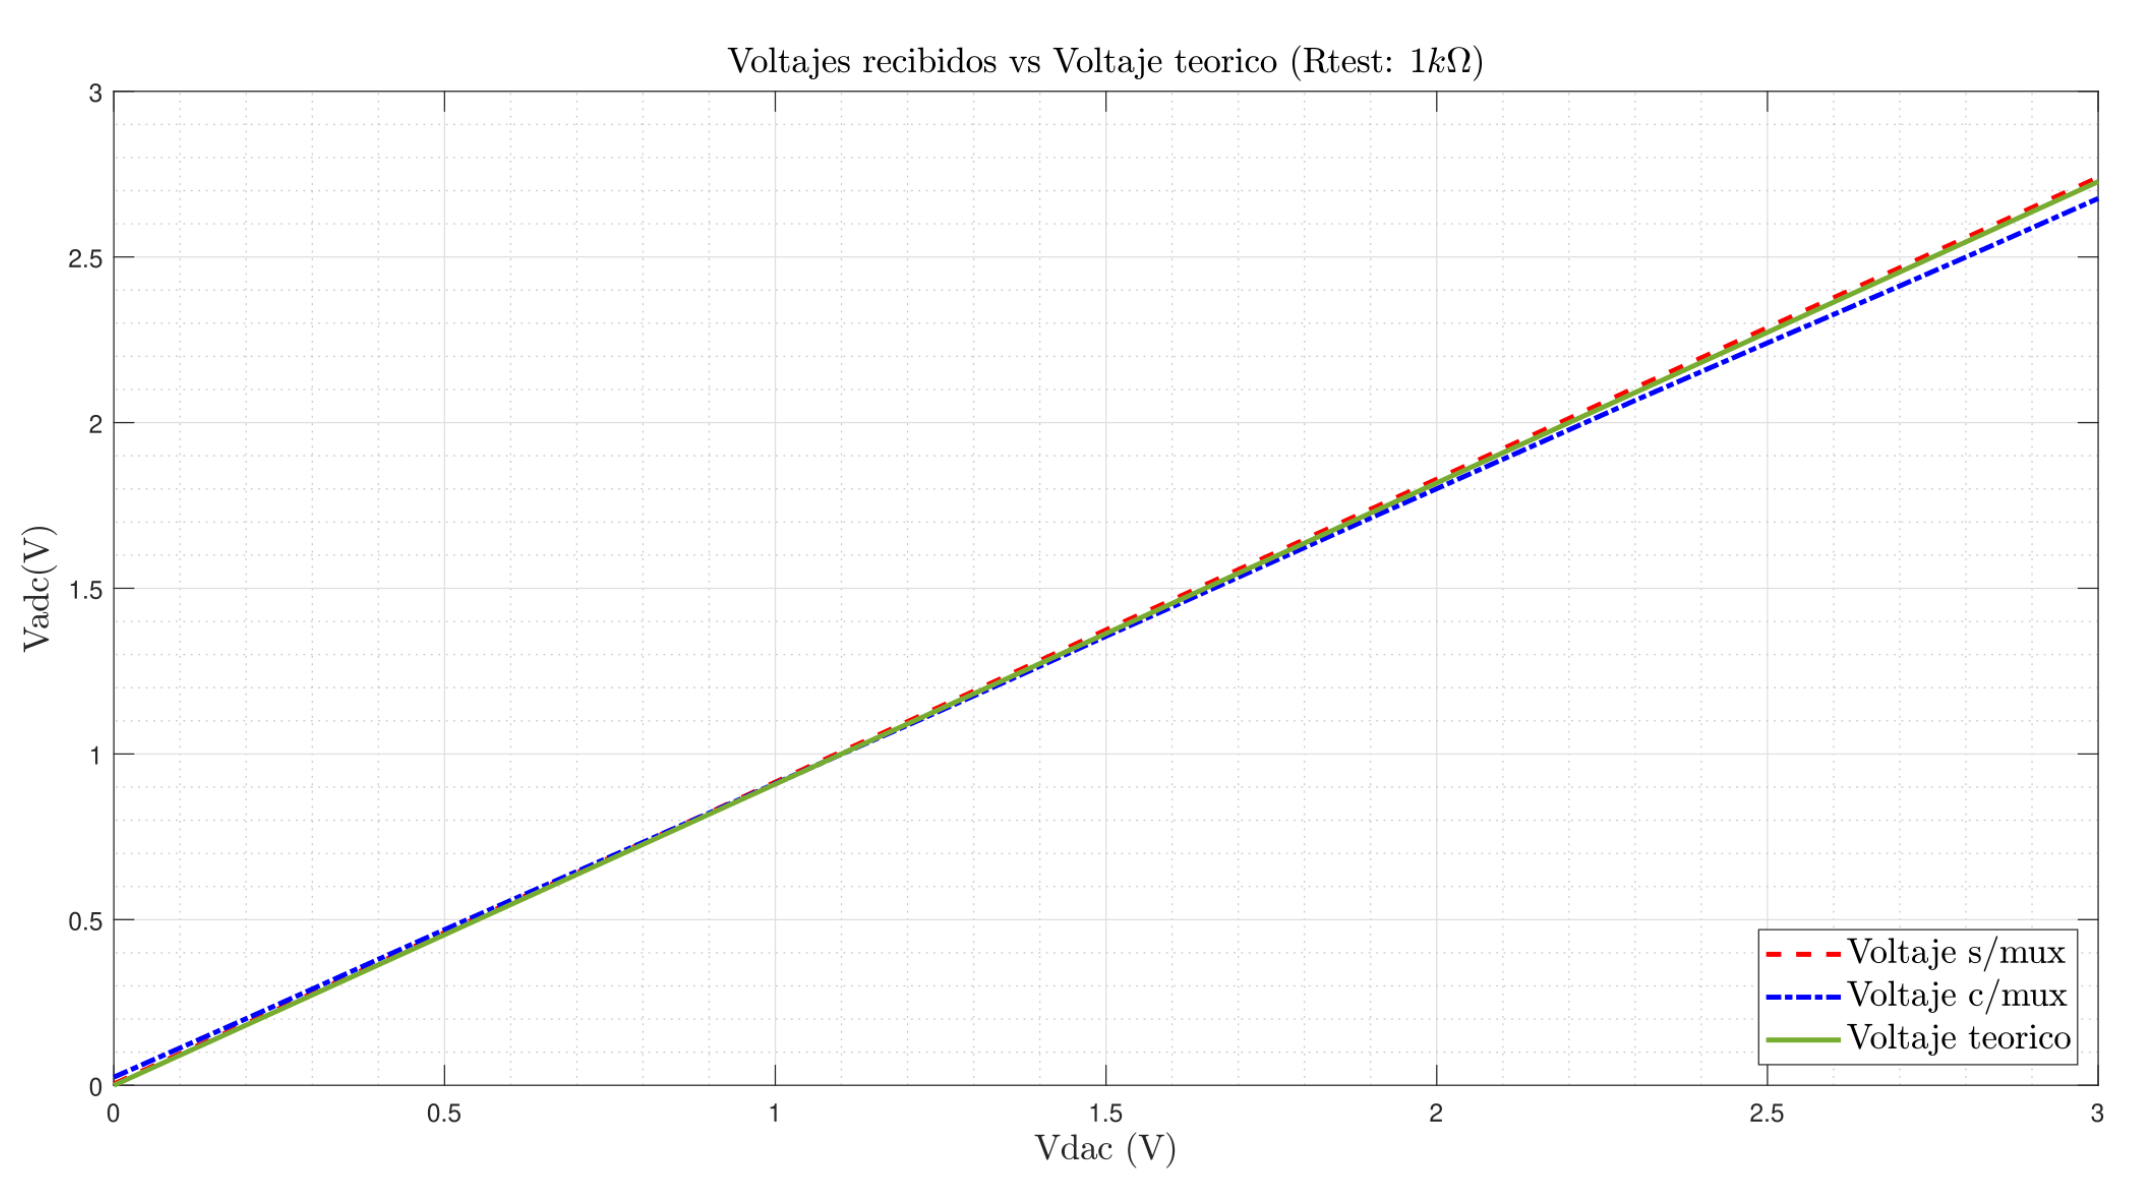
\includegraphics[width=1\textwidth]{01_1k}
                \caption{Influencia de resistencia de multiplexores.}
                \label{fig:01_1k}
            \end{figure}  
            
            \begin{figure}[hbtp]
                \centering
                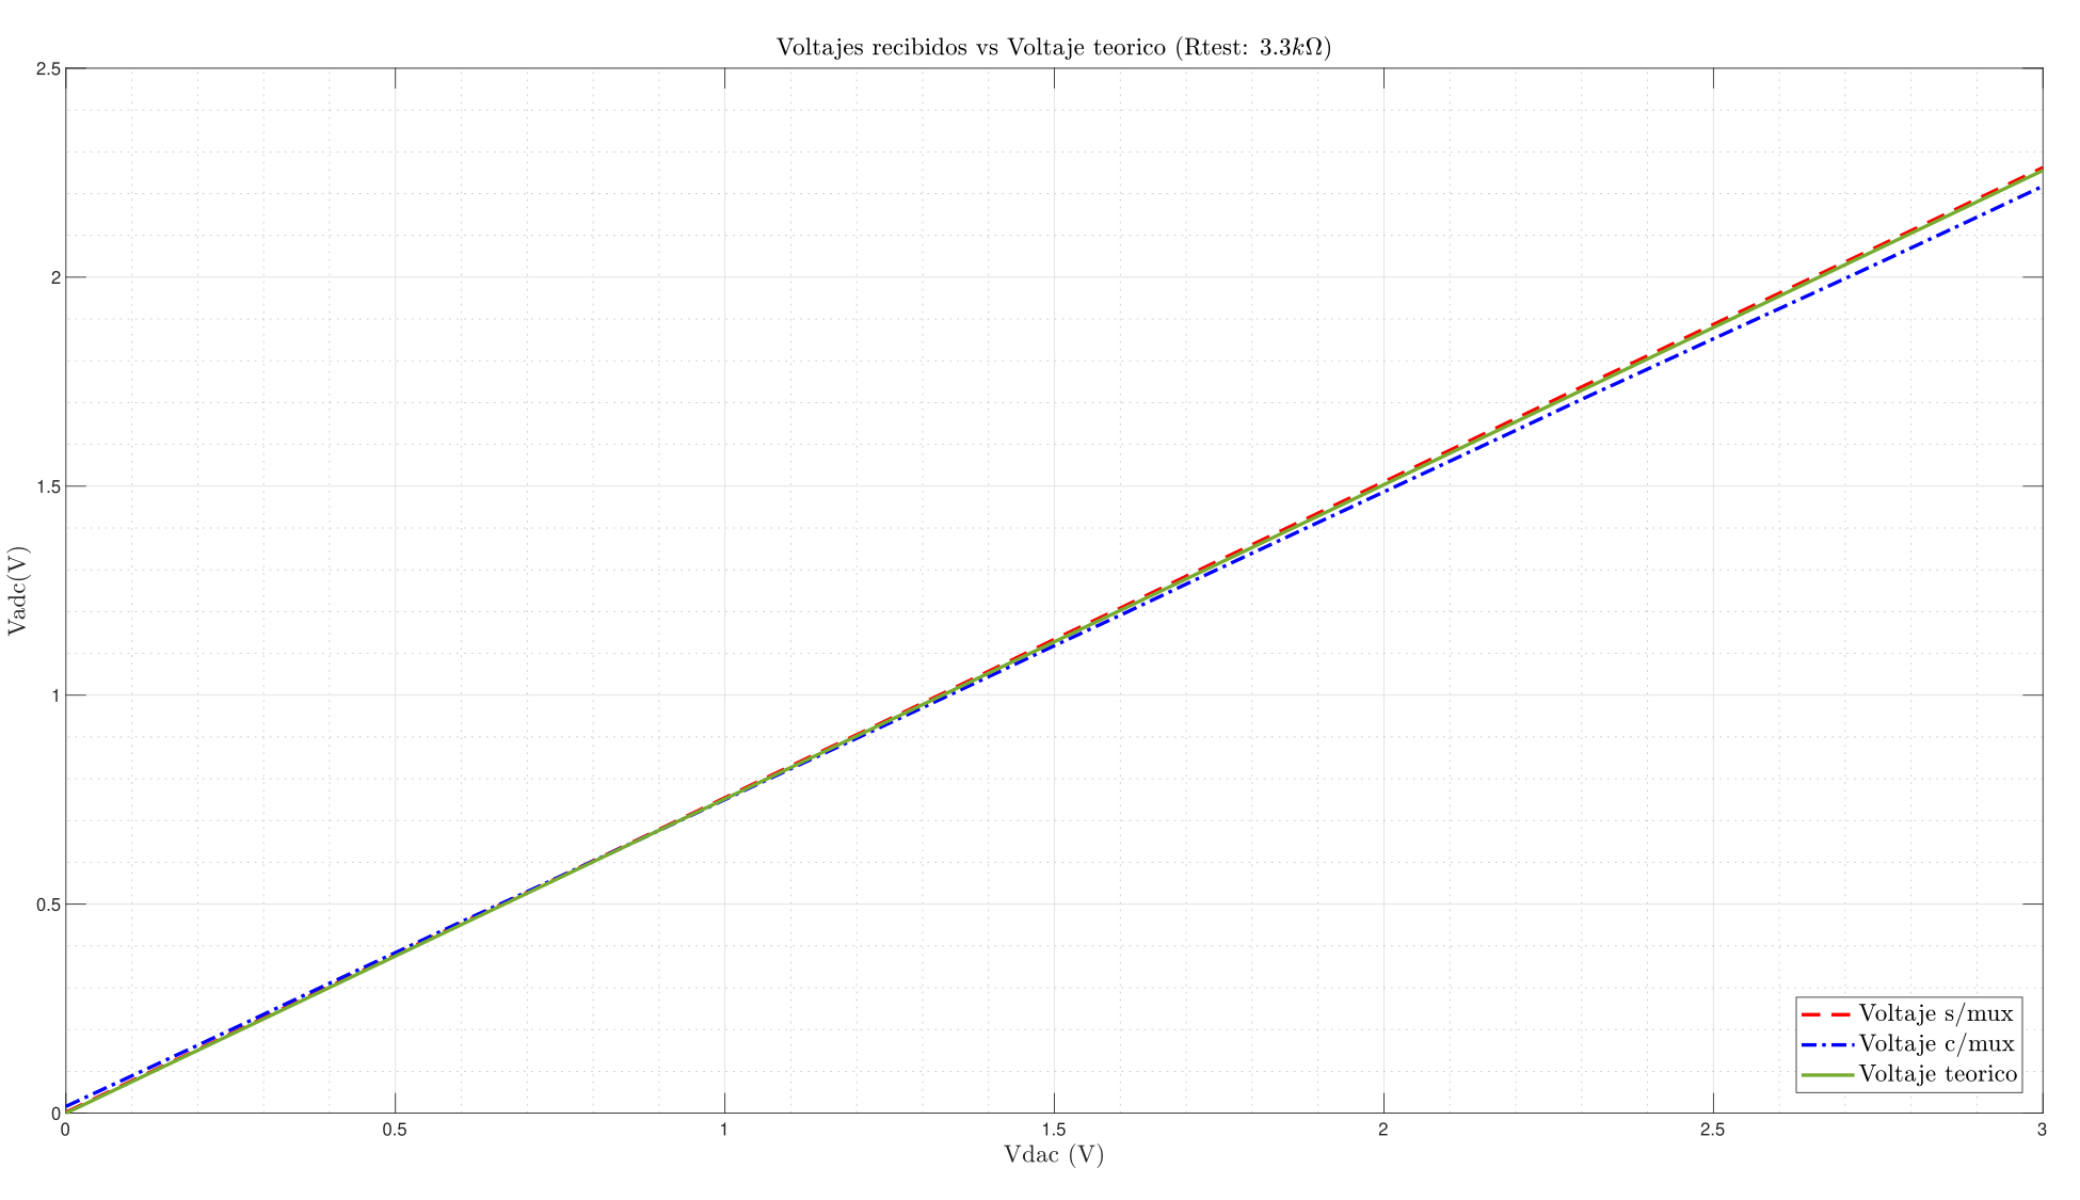
\includegraphics[width=1\textwidth]{02_3k3_new}
                \caption{Influencia de resistencia de multiplexores.}
                \label{fig:02_3k3_new}
            \end{figure}              
 
            \begin{figure}[hbtp]
                \centering
                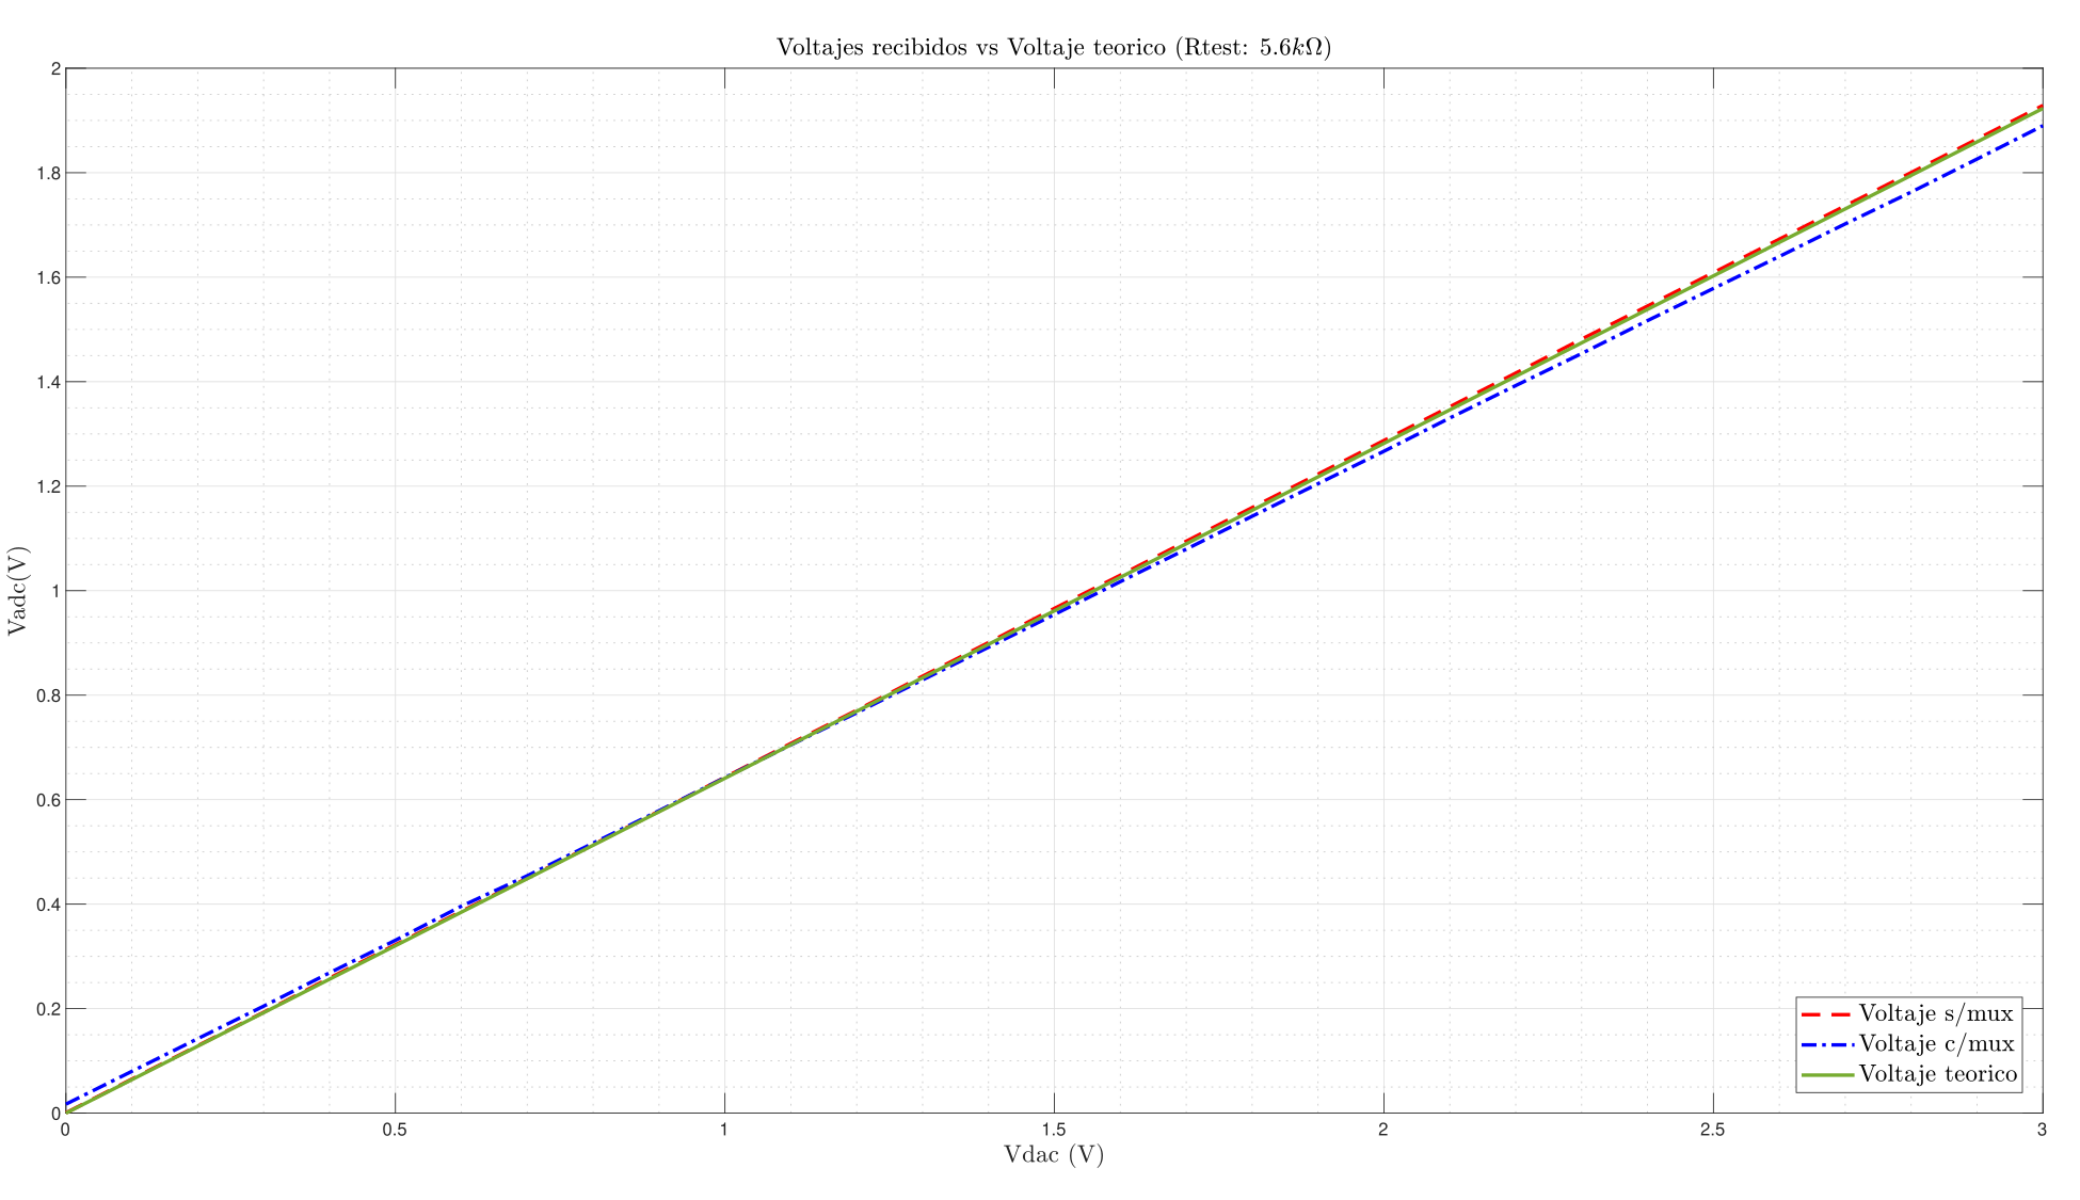
\includegraphics[width=1\textwidth]{03_5k6_new}
                \caption{Influencia de resistencia de multiplexores.}
                \label{fig:03_5k6_new}
            \end{figure}   

            \begin{figure}[hbtp]
                \centering
                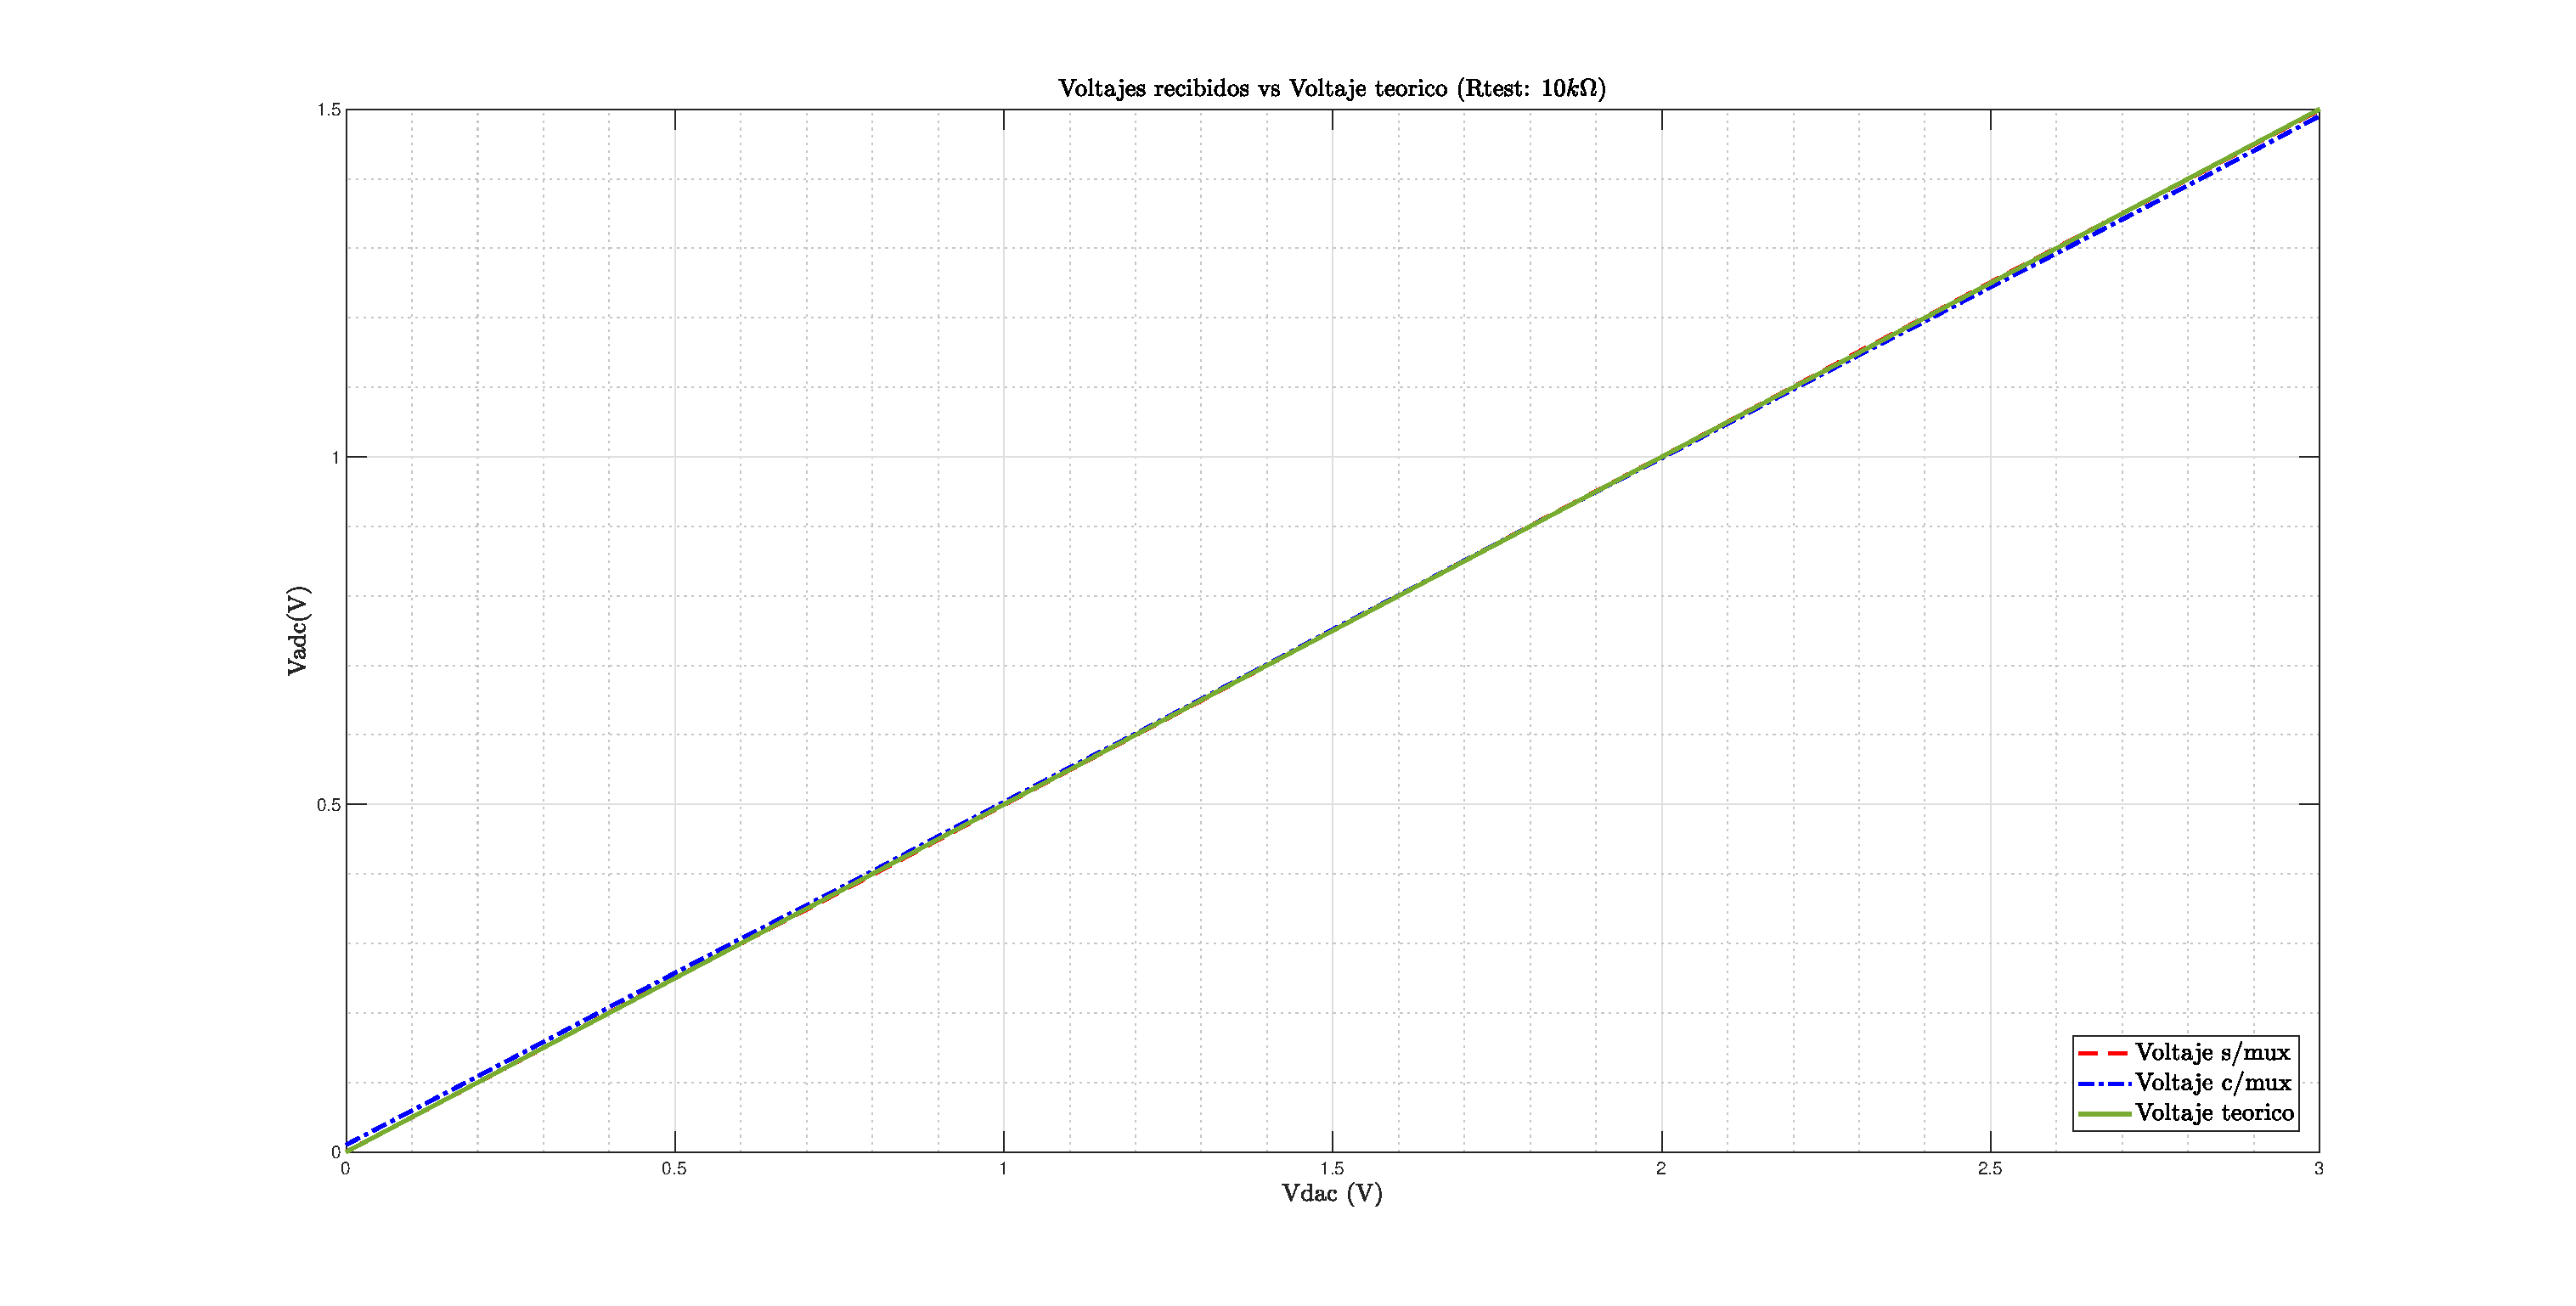
\includegraphics[width=1\textwidth]{04_10k_new}
                \caption{Influencia de resistencia de multiplexores.}
                \label{fig:04_10k_new}
            \end{figure}  
                
\newpage                      
\section{Resultados de caracterización de fotorresistencias}

            \begin{table}[htbp]
                \caption{Valor de fotorresistencias con diferentes duty cycles.}
                \begin{center}
                    \resizebox{0.6\linewidth}{!}{ 
                    \begin{NiceTabular}{| c | c | c |}
                        \CodeBefore
                        \Body
                        \hline
                        \textbf{$V_{Fuente}$}  & \textbf{Duty cycle ($\%$)} & \textbf{$R_{med} (K\Omega)$} \\
                        \hline
                        3 V     & 25  & 210 - 213.7\\
                                & 50  & 104 - 105.7\\
                                & 75  & 70 -71\\
                                & 100 & 53 - 54\\ \hline
                        3.3 V   & 25  & 29 - 31\\
                                & 50  & 16 - 17\\
                                & 75  & 11 - 12\\
                                & 100 & 8 - 9\\ \hline
                        3.5 V   & 25  & 6 - 7\\
                                & 50  & 3.6\\
                                & 75  & 2.6\\
                                & 100 & 2\\                             
                        \hline
                    \end{NiceTabular}
                    }
                \label{tab:Duty_cycle}
                \end{center}
            \end{table}


            \begin{figure}[hbtp]
                \centering
                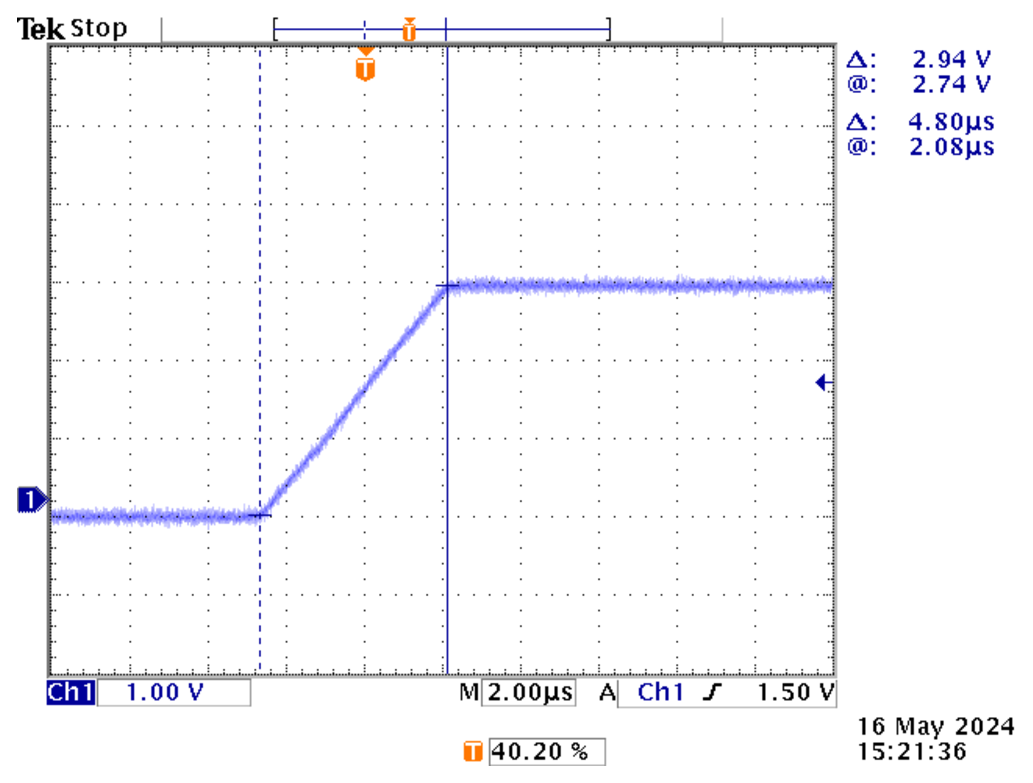
\includegraphics[width=0.6\textwidth]{settling_3v}
                \caption{Captura de osciloscopio de settling time.}
                \label{fig:settling_3v}
            \end{figure}
            
            \begin{figure}[hbtp]
                \centering
                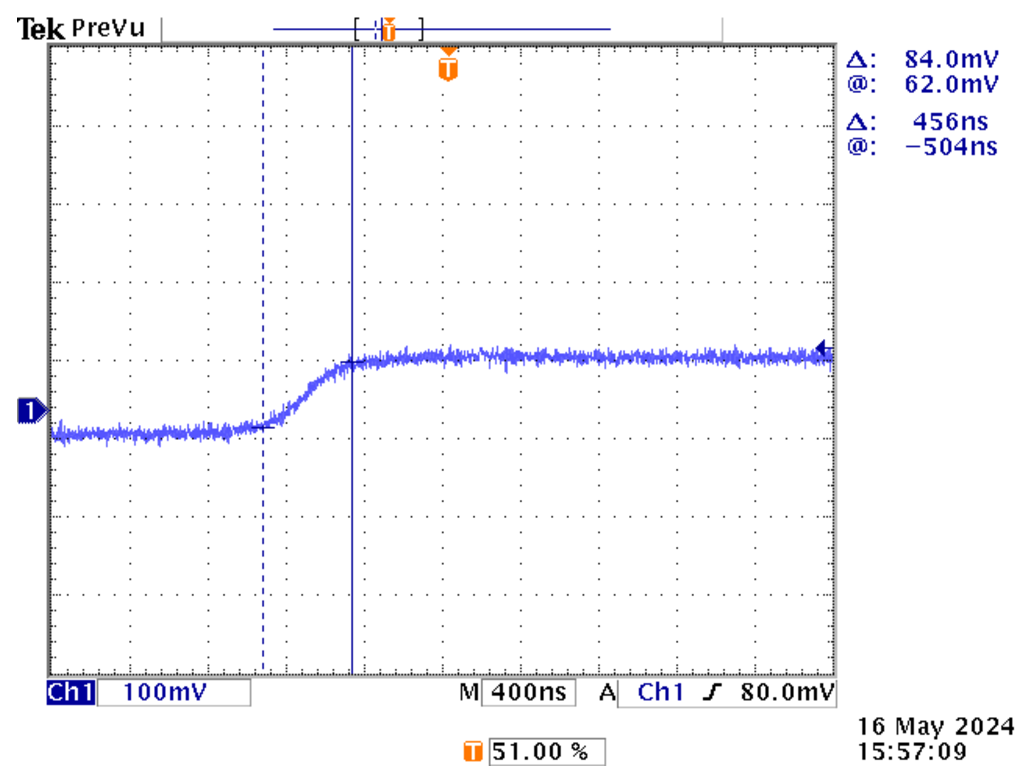
\includegraphics[width=0.6\textwidth]{settling_0v1}
                \caption{Captura de osciloscopio de settling time.}
                \label{fig:settling_0v1}
            \end{figure} 
            
            \begin{figure}[hbtp]
                \centering
                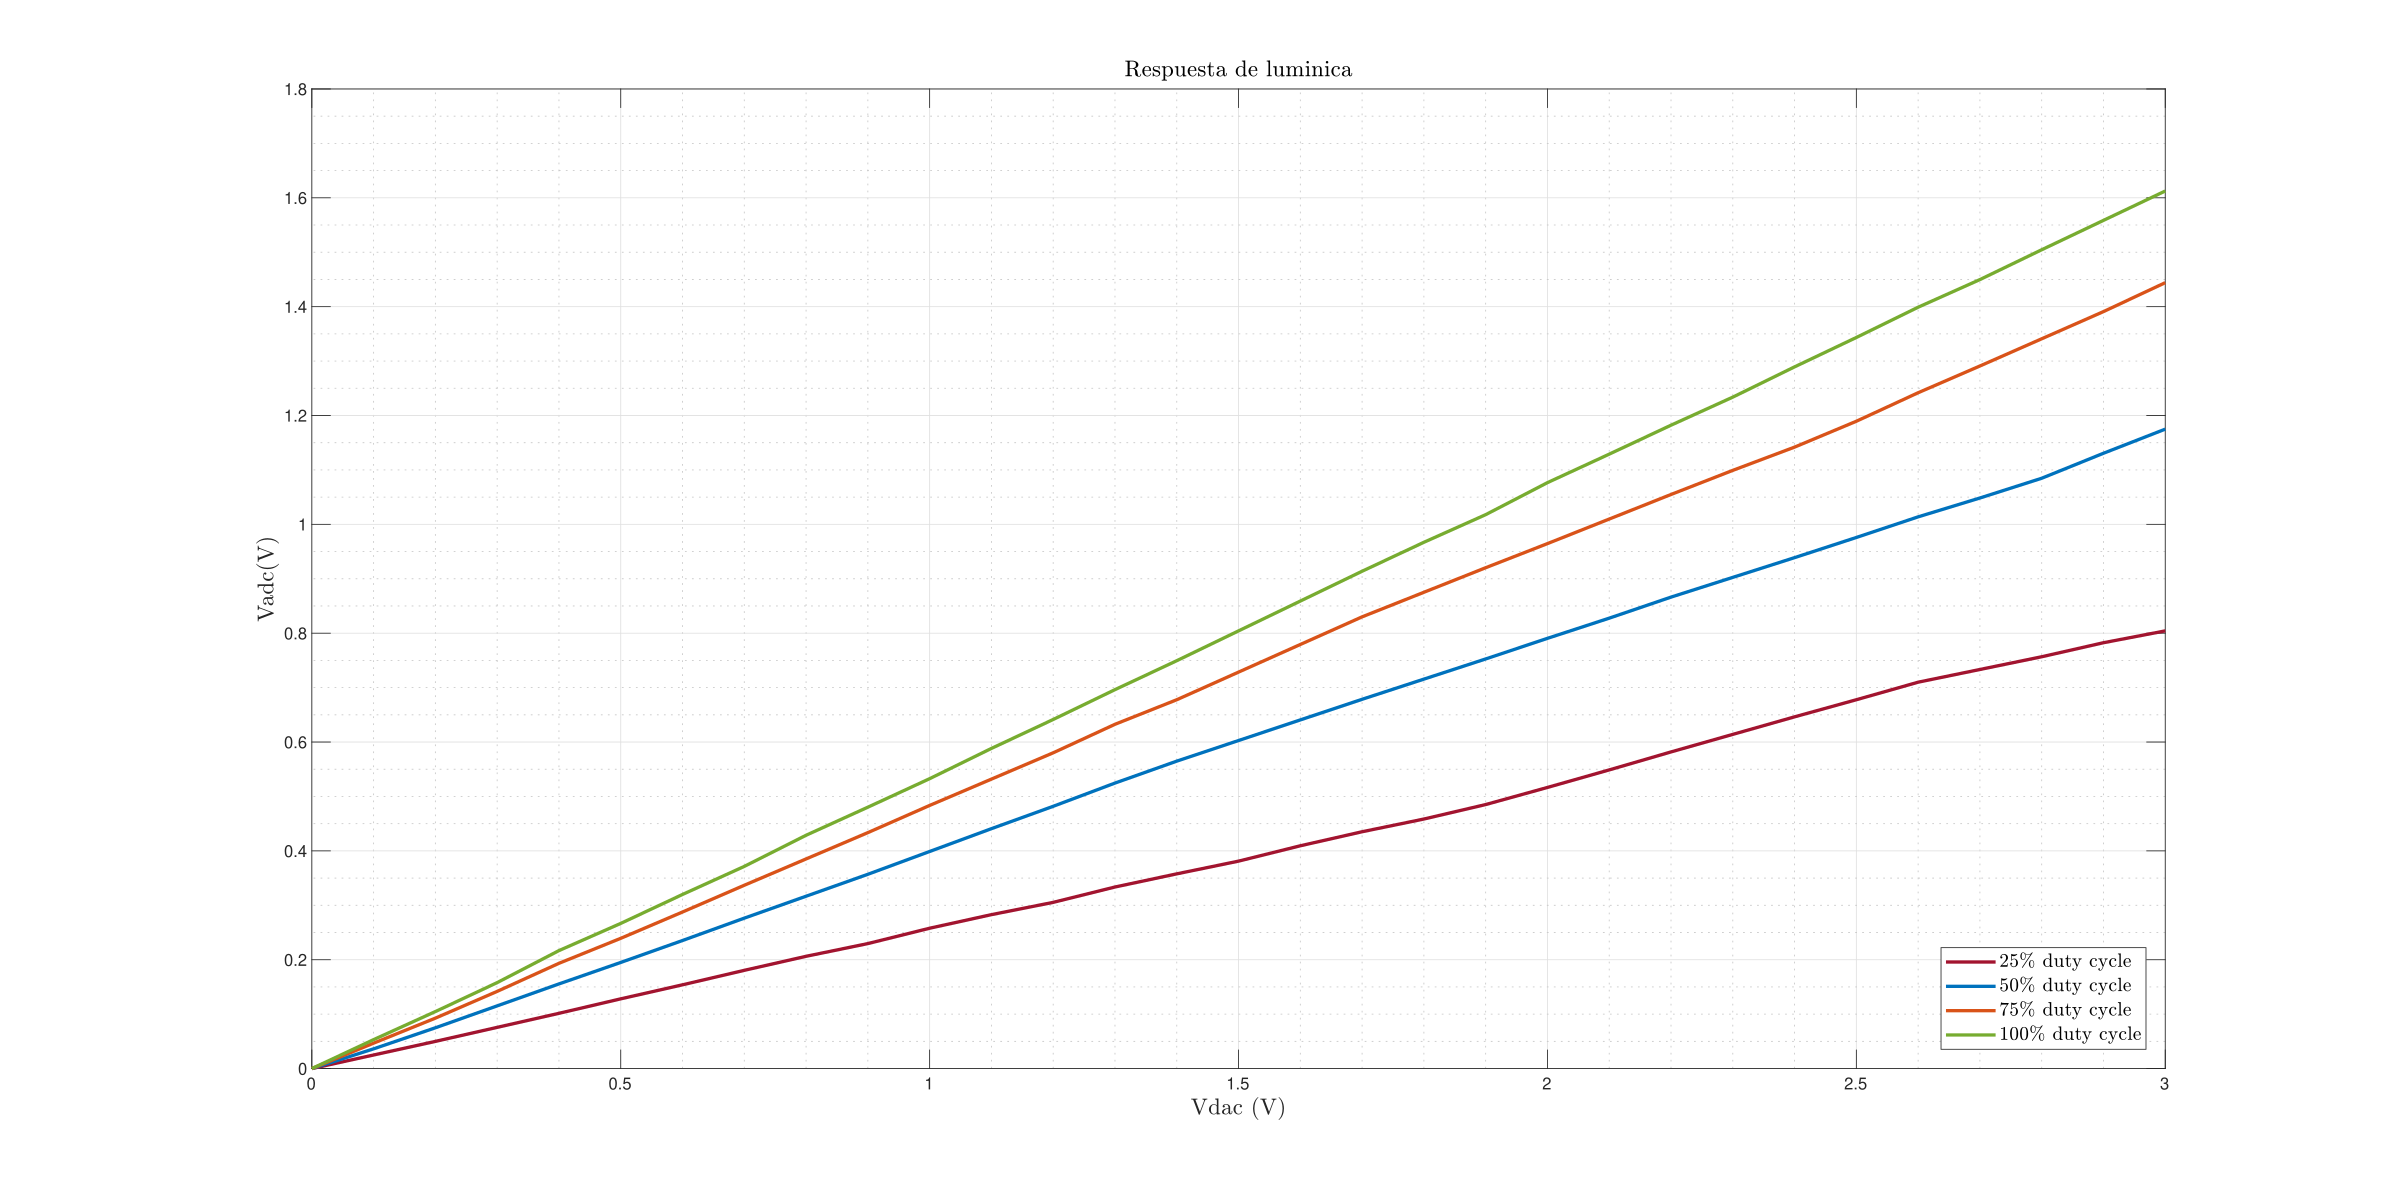
\includegraphics[width=1\textwidth]{respuesta_luminica}
                \caption{Respuesta lumínica.}
                \label{fig:respuesta_luminica}
            \end{figure}            
            
            
\newpage
\section{Imágenes obtenidas}

            \begin{figure}[hbtp]
                \centering
                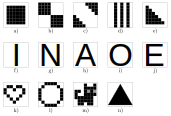
\includegraphics[width=0.8\textwidth]{mask_final}
                \caption{Máscaras aplicadas a matriz de fototransistores.}
                \label{fig:mask_final}
            \end{figure}  
\newpage
\subsection{Cuadrado}

            \begin{figure}[hbtp]
                \centering
                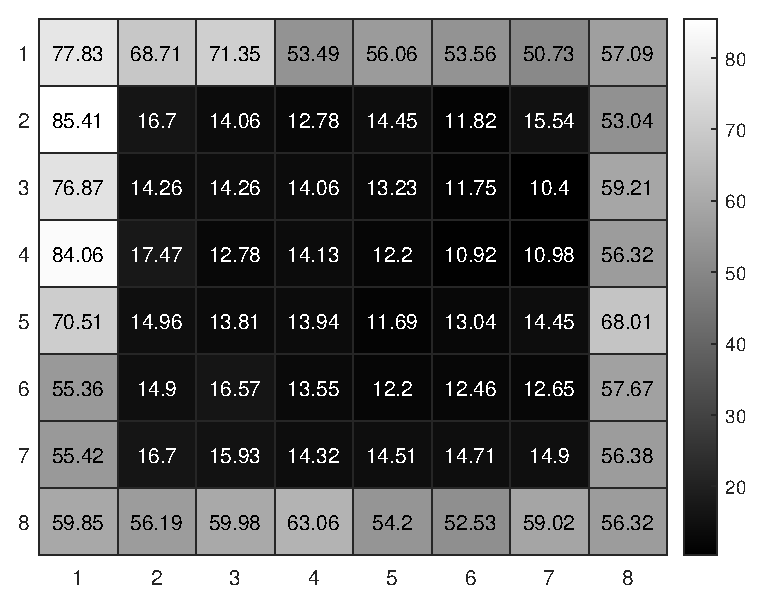
\includegraphics[width=0.6\textwidth]{fig_02}
                \caption{Máscaras aplicadas a matriz de fototransistores.}
                \label{fig:fig_02}
            \end{figure} 
\newpage            
\subsection{Cuadrados contra esquina}

            \begin{figure}[hbtp]
                \centering
                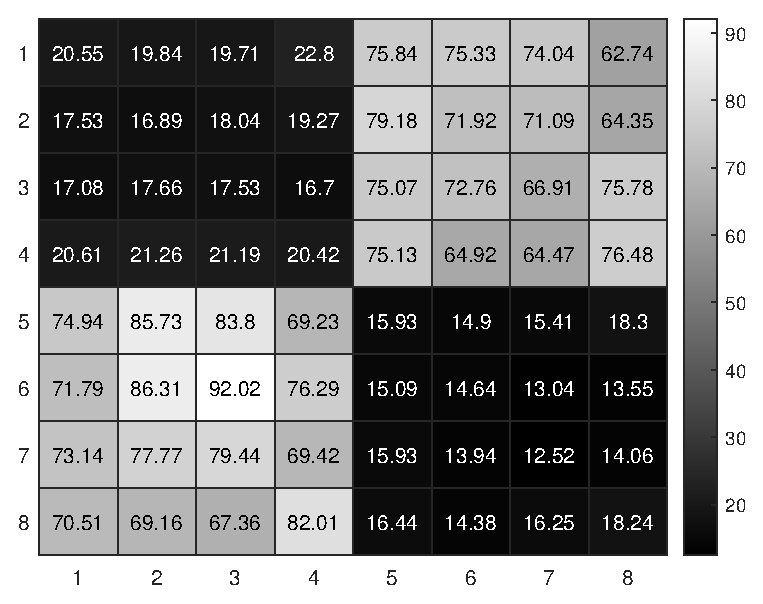
\includegraphics[width=0.6\textwidth]{fig_01}
                \caption{Máscaras aplicadas a matriz de fototransistores.}
                \label{fig:fig_01}
            \end{figure} 
\newpage
\subsection{Escaleras contra esquina}

            \begin{figure}[hbtp]
                \centering
                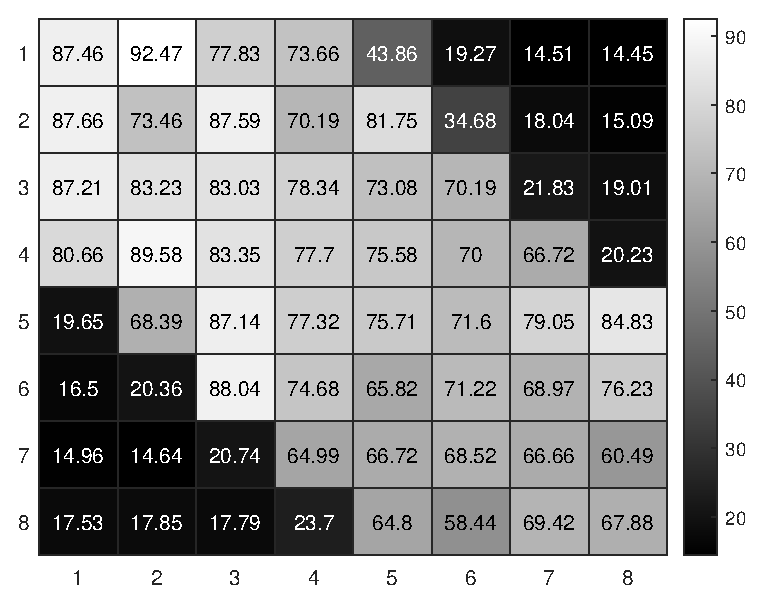
\includegraphics[width=0.6\textwidth]{fig_08}
                \caption{Máscaras aplicadas a matriz de fototransistores.}
                \label{fig:fig_08}
            \end{figure} 
\newpage
\subsection{Líneas}

            \begin{figure}[hbtp]
                \centering
                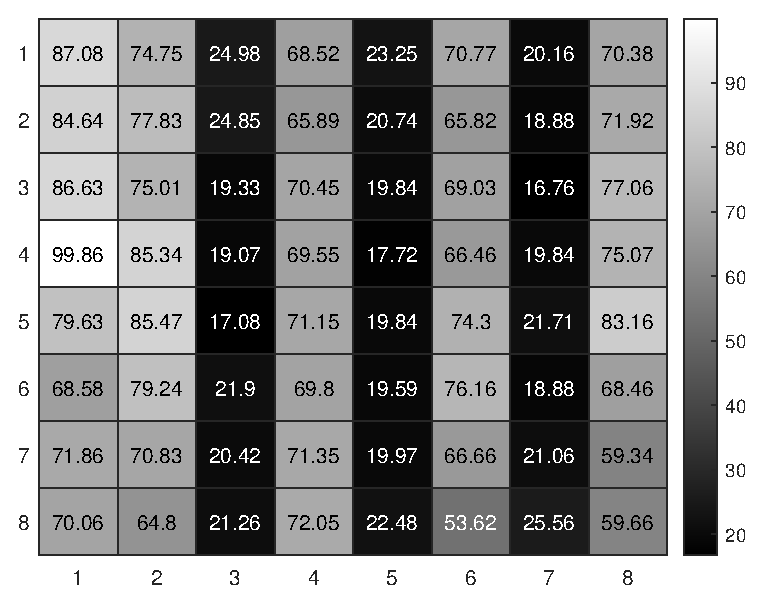
\includegraphics[width=0.6\textwidth]{fig_05}
                \caption{Máscaras aplicadas a matriz de fototransistores.}
                \label{fig:fig_05}
            \end{figure} 
\newpage
\subsection{Escalera}

            \begin{figure}[hbtp]
                \centering
                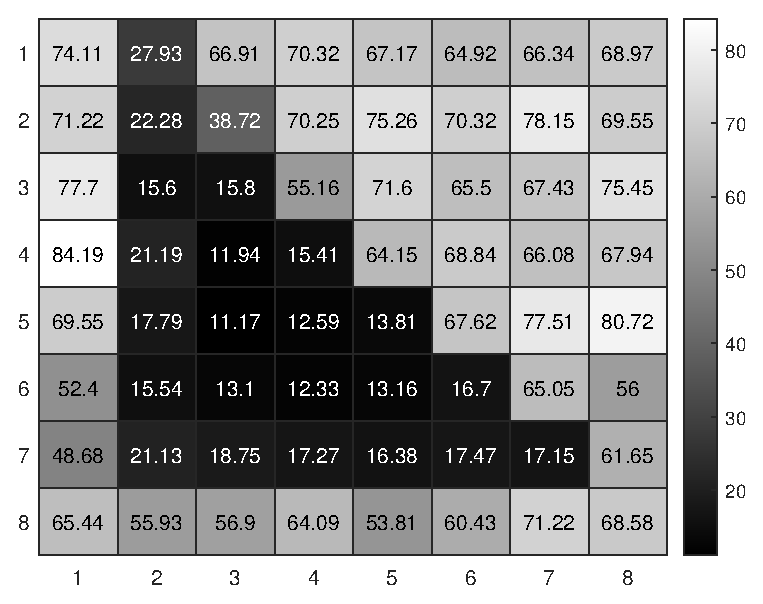
\includegraphics[width=0.6\textwidth]{fig_06}
                \caption{Máscaras aplicadas a matriz de fototransistores.}
                \label{fig:fig_06}
            \end{figure} 
\newpage
\subsection{Letra I}

            \begin{figure}[hbtp]
                \centering
                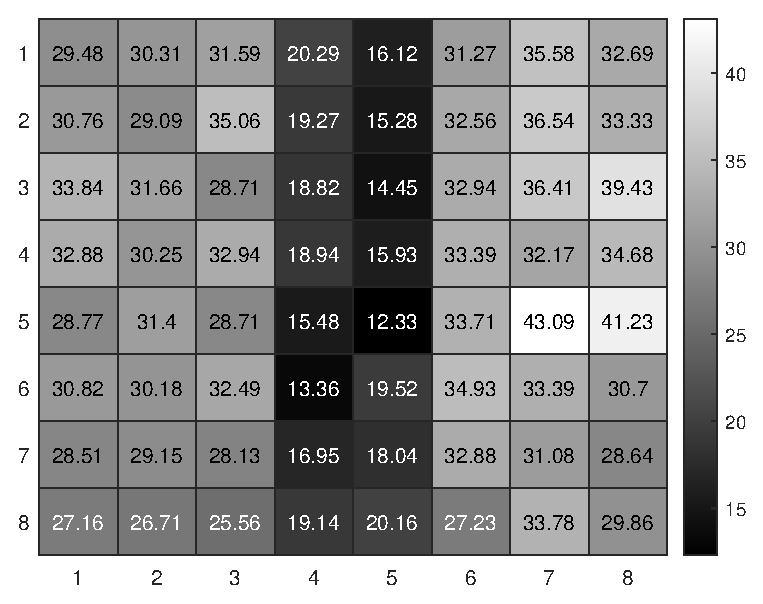
\includegraphics[width=0.6\textwidth]{01_i}
                \caption{Máscaras aplicadas a matriz de fototransistores.}
                \label{fig:01_i}
            \end{figure} 
\newpage
\subsection{Letra N}

            \begin{figure}[hbtp]
                \centering
                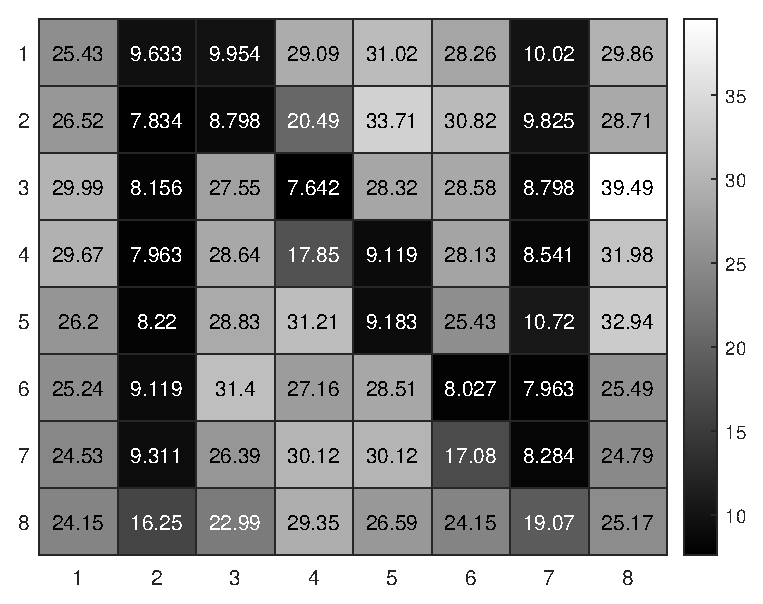
\includegraphics[width=0.6\textwidth]{02_n}
                \caption{Máscaras aplicadas a matriz de fototransistores.}
                \label{fig:02_n}
            \end{figure} 
\newpage
\subsection{Letra A}

            \begin{figure}[hbtp]
                \centering
                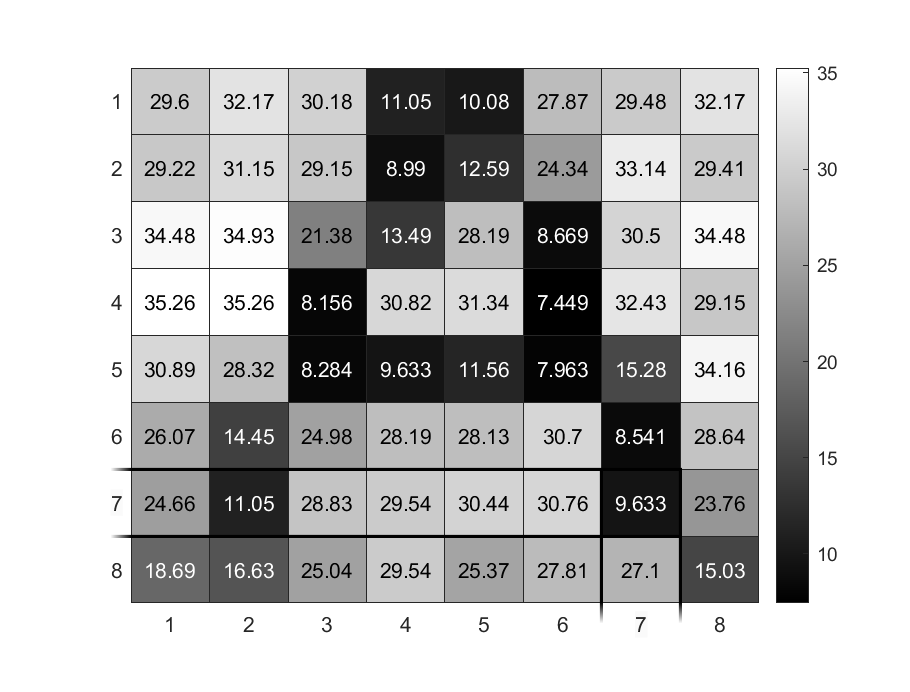
\includegraphics[width=0.6\textwidth]{03_a}
                \caption{Máscaras aplicadas a matriz de fototransistores.}
                \label{fig:03_a}
            \end{figure} 
\newpage
\subsection{Letra O}

            \begin{figure}[hbtp]
                \centering
                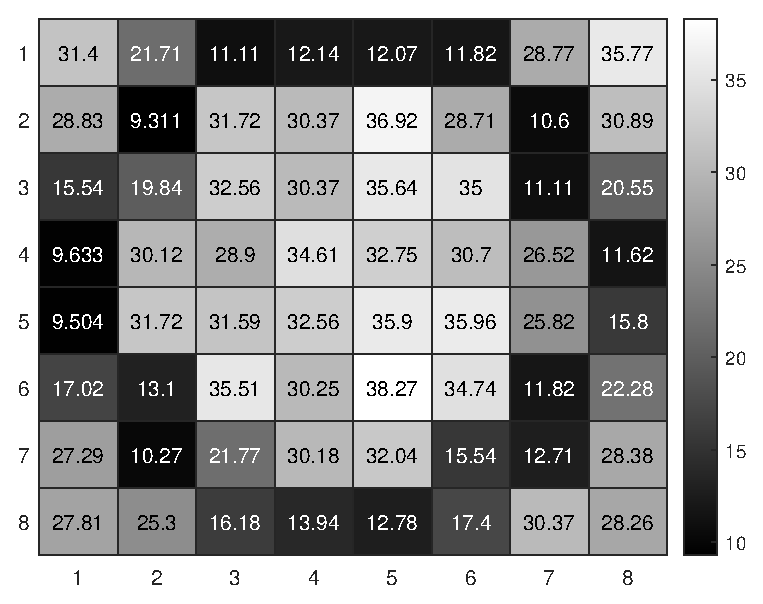
\includegraphics[width=0.6\textwidth]{04_o}
                \caption{Máscaras aplicadas a matriz de fototransistores.}
                \label{fig:04_o}
            \end{figure} 
\newpage
\subsection{Letra E}

            \begin{figure}[hbtp]
                \centering
                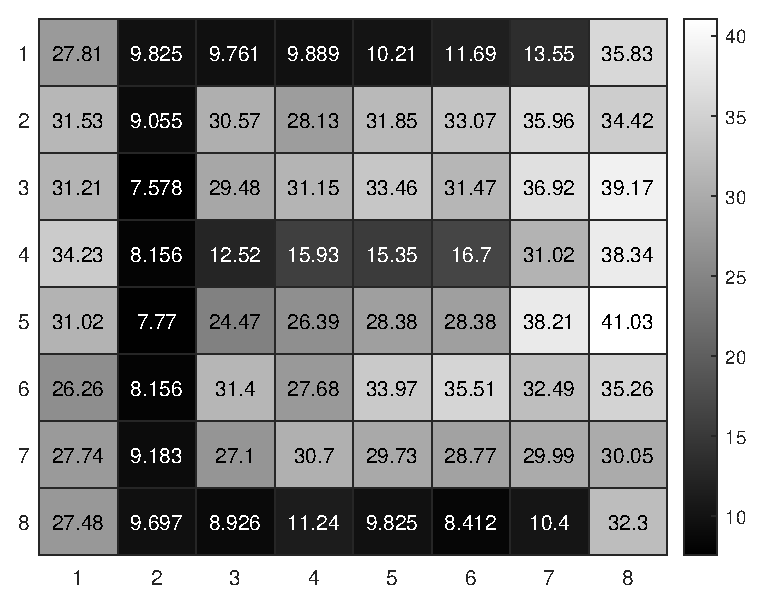
\includegraphics[width=0.6\textwidth]{05_e}
                \caption{Máscaras aplicadas a matriz de fototransistores.}
                \label{fig:05_e}
            \end{figure} 
\newpage
\subsection{Corazón}

            \begin{figure}[hbtp]
                \centering
                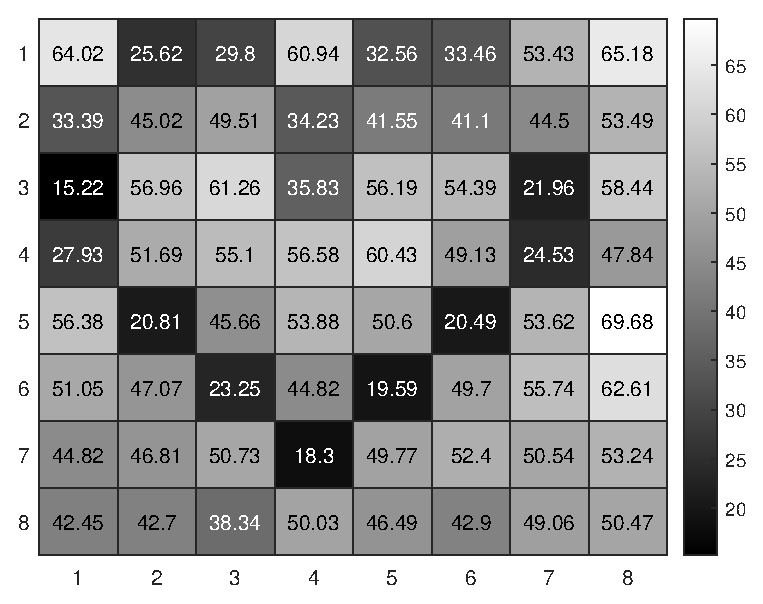
\includegraphics[width=0.6\textwidth]{fig_04}
                \caption{Máscaras aplicadas a matriz de fototransistores.}
                \label{fig:fig_04}
            \end{figure} 
\newpage
\subsection{Círculo}

            \begin{figure}[hbtp]
                \centering
                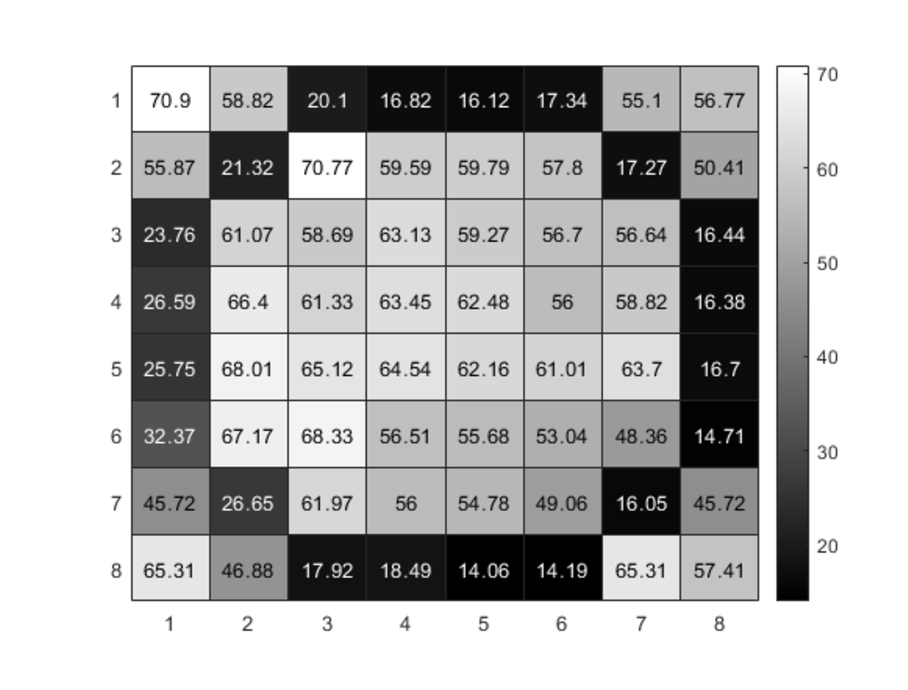
\includegraphics[width=0.6\textwidth]{circle}
                \caption{Máscaras aplicadas a matriz de fototransistores.}
                \label{fig:circle}
            \end{figure} 
\newpage
\subsection{Gato}

            \begin{figure}[hbtp]
                \centering
                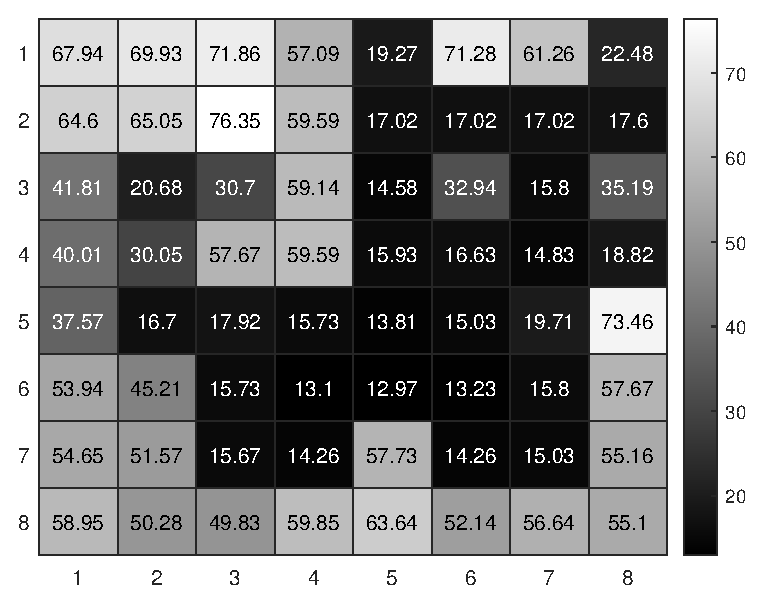
\includegraphics[width=0.6\textwidth]{fig_07}
                \caption{Máscaras aplicadas a matriz de fototransistores.}
                \label{fig:fig_07}
            \end{figure} 
\newpage
\subsection{Triángulo}

            \begin{figure}[hbtp]
                \centering
                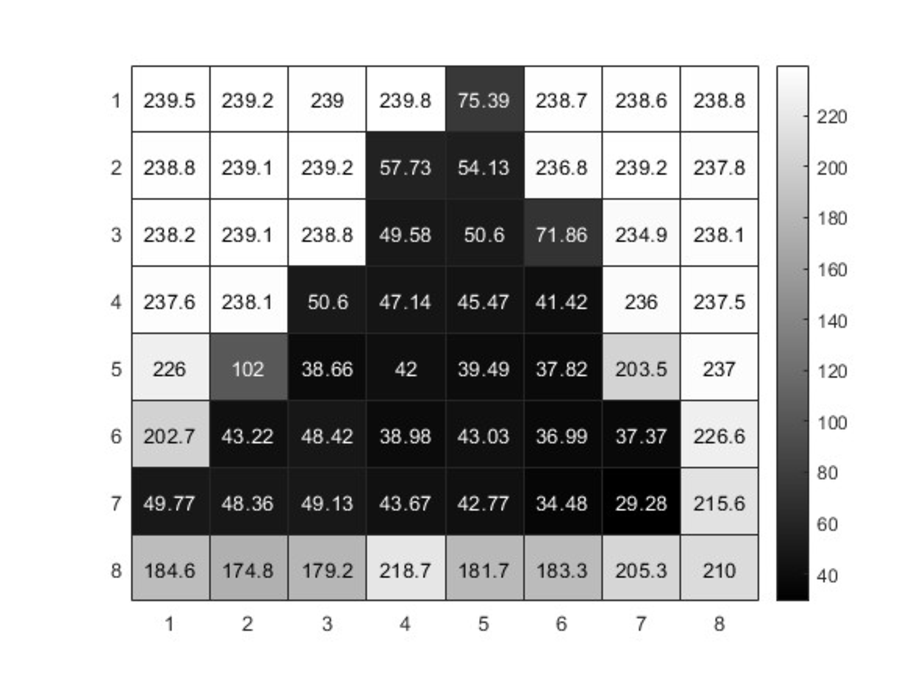
\includegraphics[width=0.6\textwidth]{triangle}
                \caption{Máscaras aplicadas a matriz de fototransistores.}
                \label{fig:triangle}
            \end{figure} 
